%%%%%%%%%%%%%%%%%%%%%%%%%%%%%%%%%%%%%%%%%
% The Legrand Orange Book
% LaTeX Template
% Version 2.3 (8/8/17)
%
%
% License:
% CC BY-NC-SA 3.0 (http://creativecommons.org/licenses/by-nc-sa/3.0/)
%
% Compiling this template:
% This template uses biber for its bibliography and makeindex for its index.
% When you first open the template, compile it from the command line with the 
% commands below to make sure your LaTeX distribution is configured correctly:
%
% 1) pdflatex main
% 2) makeindex main.idx -s StyleInd.ist
% 3) biber main
% 4) pdflatex main x 2
%
% After this, when you wish to update the bibliography/index use the appropriate
% command above and make sure to compile with pdflatex severa
% This template has been downloaded from:
% http://www.LaTeXTemplates.com
% This template also uses a number of packages which may need to be
% updated to the newest versions for the template to compile. It is strongly
% recommended you update your LaTeX distribution if you have any
% compilation errors.
%
% Important note:
% Chapter heading images should have a 2:1 width:height ratio,
% e.g. 920px width and 460px height.
%
%%%%%%%%%%%%%%%%%%%%%%%%%%%%%%%%%%%%%%%%%

%----------------------------------------------------------------------------------------
%	PACKAGES AND OTHER DOCUMENT CONFIGURATIONS
%----------------------------------------------------------------------------------------

\documentclass[11pt,fleqn]{book} % Default font size and left-justified equations

%----------------------------------------------------------------------------------------
\usepackage{listings}
\usepackage{xcolor}
\usepackage{caption}
\usepackage{makecell}
\usepackage{tikz}
\usepackage{float}
\usetikzlibrary{arrows, chains}
\lstset {
	language=C++,
	backgroundcolor=\color{black!5},
	basicstyle=\footnotesize,
	frame=tb,
	tabsize=4,
	showstringspaces=false,
	commentstyle=\color{green},
	keywordstyle=\color{blue},
	stringstyle=\color{red},
}
%%%%%%%%%%%%%%%%%%%%%%%%%%%%%%%%%%%%%%%%%
% The Legrand Orange Book
% Structural Definitions File
% Version 2.0 (9/2/15)
%
% Original author:
% Mathias Legrand (legrand.mathias@gmail.com) with modifications by:
% Vel (vel@latextemplates.com)
% 
% This file has been downloaded from:
% http://www.LaTeXTemplates.com
%
% License:
% CC BY-NC-SA 3.0 (http://creativecommons.org/licenses/by-nc-sa/3.0/)
%
%%%%%%%%%%%%%%%%%%%%%%%%%%%%%%%%%%%%%%%%%

%----------------------------------------------------------------------------------------
%	VARIOUS REQUIRED PACKAGES AND CONFIGURATIONS
%----------------------------------------------------------------------------------------

\usepackage[top=3cm,bottom=3cm,left=3cm,right=3cm,headsep=10pt,a4paper]{geometry} % Page margins

\usepackage{graphicx} % Required for including pictures
\graphicspath{{Pictures/}} % Specifies the directory where pictures are stored

\usepackage{lipsum} % Inserts dummy text

\usepackage{tikz} % Required for drawing custom shapes

\usepackage[english]{babel} % English language/hyphenation

\usepackage{enumitem} % Customize lists
\setlist{nolistsep} % Reduce spacing between bullet points and numbered lists

\usepackage{booktabs} % Required for nicer horizontal rules in tables

\usepackage{xcolor} % Required for specifying colors by name
\definecolor{ocre}{RGB}{225,100,225} % Define the orange color used for highlighting throughout the book

%----------------------------------------------------------------------------------------
%	FONTS
%----------------------------------------------------------------------------------------

\usepackage{avant} % Use the Avantgarde font for headings
%\usepackage{times} % Use the Times font for headings
\usepackage{mathptmx} % Use the Adobe Times Roman as the default text font together with math symbols from the Sym­bol, Chancery and Com­puter Modern fonts

\usepackage{microtype} % Slightly tweak font spacing for aesthetics
\usepackage[utf8]{inputenc} % Required for including letters with accents
\usepackage[T1]{fontenc} % Use 8-bit encoding that has 256 glyphs

%----------------------------------------------------------------------------------------
%	BIBLIOGRAPHY AND INDEX
%----------------------------------------------------------------------------------------

\usepackage[style=numeric,citestyle=numeric,sorting=nyt,sortcites=true,autopunct=true,babel=hyphen,hyperref=true,abbreviate=false,backref=true,backend=biber]{biblatex}
\addbibresource{bibliography.bib} % BibTeX bibliography file
\defbibheading{bibempty}{}

\usepackage{calc} % For simpler calculation - used for spacing the index letter headings correctly
\usepackage{makeidx} % Required to make an index
\makeindex % Tells LaTeX to create the files required for indexing

%----------------------------------------------------------------------------------------
%	MAIN TABLE OF CONTENTS
%----------------------------------------------------------------------------------------

\usepackage{titletoc} % Required for manipulating the table of contents

\contentsmargin{0cm} % Removes the default margin

% Part text styling
\titlecontents{part}[0cm]
{\addvspace{20pt}\centering\large\bfseries}
{}
{}
{}

% Chapter text styling
\titlecontents{chapter}[1.25cm] % Indentation
{\addvspace{12pt}\large\sffamily\bfseries} % Spacing and font options for chapters
{\color{ocre!60}\contentslabel[\Large\thecontentslabel]{1.25cm}\color{ocre}} % Chapter number
{\color{ocre}}  
{\color{ocre!60}\normalsize\;\titlerule*[.5pc]{.}\;\thecontentspage} % Page number

% Section text styling
\titlecontents{section}[1.25cm] % Indentation
{\addvspace{3pt}\sffamily\bfseries} % Spacing and font options for sections
{\contentslabel[\thecontentslabel]{1.25cm}} % Section number
{}
{\hfill\color{black}\thecontentspage} % Page number
[]

% Subsection text styling
\titlecontents{subsection}[1.25cm] % Indentation
{\addvspace{1pt}\sffamily\small} % Spacing and font options for subsections
{\contentslabel[\thecontentslabel]{1.25cm}} % Subsection number
{}
{\ \titlerule*[.5pc]{.}\;\thecontentspage} % Page number
[]

% List of figures
\titlecontents{figure}[0em]
{\addvspace{-5pt}\sffamily}
{\thecontentslabel\hspace*{1em}}
{}
{\ \titlerule*[.5pc]{.}\;\thecontentspage}
[]

% List of tables
\titlecontents{table}[0em]
{\addvspace{-5pt}\sffamily}
{\thecontentslabel\hspace*{1em}}
{}
{\ \titlerule*[.5pc]{.}\;\thecontentspage}
[]

%----------------------------------------------------------------------------------------
%	MINI TABLE OF CONTENTS IN PART HEADS
%----------------------------------------------------------------------------------------

% Chapter text styling
\titlecontents{lchapter}[0em] % Indenting
{\addvspace{15pt}\large\sffamily\bfseries} % Spacing and font options for chapters
{\color{ocre}\contentslabel[\Large\thecontentslabel]{1.25cm}\color{ocre}} % Chapter number
{}  
{\color{ocre}\normalsize\sffamily\bfseries\;\titlerule*[.5pc]{.}\;\thecontentspage} % Page number

% Section text styling
\titlecontents{lsection}[0em] % Indenting
{\sffamily\small} % Spacing and font options for sections
{\contentslabel[\thecontentslabel]{1.25cm}} % Section number
{}
{}

% Subsection text styling
\titlecontents{lsubsection}[.5em] % Indentation
{\normalfont\footnotesize\sffamily} % Font settings
{}
{}
{}

%----------------------------------------------------------------------------------------
%	PAGE HEADERS
%----------------------------------------------------------------------------------------

\usepackage{fancyhdr} % Required for header and footer configuration

\pagestyle{fancy}
\renewcommand{\chaptermark}[1]{\markboth{\sffamily\normalsize\bfseries\chaptername\ \thechapter.\ #1}{}} % Chapter text font settings
\renewcommand{\sectionmark}[1]{\markright{\sffamily\normalsize\thesection\hspace{5pt}#1}{}} % Section text font settings
\fancyhf{} \fancyhead[LE,RO]{\sffamily\normalsize\thepage} % Font setting for the page number in the header
\fancyhead[LO]{\rightmark} % Print the nearest section name on the left side of odd pages
\fancyhead[RE]{\leftmark} % Print the current chapter name on the right side of even pages
\renewcommand{\headrulewidth}{0.5pt} % Width of the rule under the header
\addtolength{\headheight}{2.5pt} % Increase the spacing around the header slightly
\renewcommand{\footrulewidth}{0pt} % Removes the rule in the footer
\fancypagestyle{plain}{\fancyhead{}\renewcommand{\headrulewidth}{0pt}} % Style for when a plain pagestyle is specified

% Removes the header from odd empty pages at the end of chapters
\makeatletter
\renewcommand{\cleardoublepage}{
\clearpage\ifodd\c@page\else
\hbox{}
\vspace*{\fill}
\thispagestyle{empty}
\newpage
\fi}

%----------------------------------------------------------------------------------------
%	THEOREM STYLES
%----------------------------------------------------------------------------------------

\usepackage{amsmath,amsfonts,amssymb,amsthm} % For math equations, theorems, symbols, etc

\newcommand{\intoo}[2]{\mathopen{]}#1\,;#2\mathclose{[}}
\newcommand{\ud}{\mathop{\mathrm{{}d}}\mathopen{}}
\newcommand{\intff}[2]{\mathopen{[}#1\,;#2\mathclose{]}}
\newtheorem{notation}{Notation}[chapter]

% Boxed/framed environments
\newtheoremstyle{ocrenumbox}% % Theorem style name
{0pt}% Space above
{0pt}% Space below
{\normalfont}% % Body font
{}% Indent amount
{\small\bf\sffamily\color{ocre}}% % Theorem head font
{\;}% Punctuation after theorem head
{0.25em}% Space after theorem head
{\small\sffamily\color{ocre}\thmname{#1}\nobreakspace\thmnumber{\@ifnotempty{#1}{}\@upn{#2}}% Theorem text (e.g. Theorem 2.1)
\thmnote{\nobreakspace\the\thm@notefont\sffamily\bfseries\color{black}---\nobreakspace#3.}} % Optional theorem note
\renewcommand{\qedsymbol}{$\blacksquare$}% Optional qed square

\newtheoremstyle{blacknumex}% Theorem style name
{5pt}% Space above
{5pt}% Space below
{\normalfont}% Body font
{} % Indent amount
{\small\bf\sffamily}% Theorem head font
{\;}% Punctuation after theorem head
{0.25em}% Space after theorem head
{\small\sffamily{\tiny\ensuremath{\blacksquare}}\nobreakspace\thmname{#1}\nobreakspace\thmnumber{\@ifnotempty{#1}{}\@upn{#2}}% Theorem text (e.g. Theorem 2.1)
\thmnote{\nobreakspace\the\thm@notefont\sffamily\bfseries---\nobreakspace#3.}}% Optional theorem note

\newtheoremstyle{blacknumbox} % Theorem style name
{0pt}% Space above
{0pt}% Space below
{\normalfont}% Body font
{}% Indent amount
{\small\bf\sffamily}% Theorem head font
{\;}% Punctuation after theorem head
{0.25em}% Space after theorem head
{\small\sffamily\thmname{#1}\nobreakspace\thmnumber{\@ifnotempty{#1}{}\@upn{#2}}% Theorem text (e.g. Theorem 2.1)
\thmnote{\nobreakspace\the\thm@notefont\sffamily\bfseries---\nobreakspace#3.}}% Optional theorem note

% Non-boxed/non-framed environments
\newtheoremstyle{ocrenum}% % Theorem style name
{5pt}% Space above
{5pt}% Space below
{\normalfont}% % Body font
{}% Indent amount
{\small\bf\sffamily\color{ocre}}% % Theorem head font
{\;}% Punctuation after theorem head
{0.25em}% Space after theorem head
{\small\sffamily\color{ocre}\thmname{#1}\nobreakspace\thmnumber{\@ifnotempty{#1}{}\@upn{#2}}% Theorem text (e.g. Theorem 2.1)
\thmnote{\nobreakspace\the\thm@notefont\sffamily\bfseries\color{black}---\nobreakspace#3.}} % Optional theorem note
\renewcommand{\qedsymbol}{$\blacksquare$}% Optional qed square
\makeatother

% Defines the theorem text style for each type of theorem to one of the three styles above
\newcounter{dummy} 
\numberwithin{dummy}{section}
\theoremstyle{ocrenumbox}
\newtheorem{theoremeT}[dummy]{Theorem}
\newtheorem{problem}{Problem}[chapter]
\newtheorem{exerciseT}{Exercise}[chapter]
\theoremstyle{blacknumex}
\newtheorem{exampleT}{Example}[chapter]
\theoremstyle{blacknumbox}
\newtheorem{vocabulary}{Vocabulary}[chapter]
\newtheorem{definitionT}{Definition}[section]
\newtheorem{corollaryT}[dummy]{Corollary}
\theoremstyle{ocrenum}
\newtheorem{proposition}[dummy]{Proposition}

%----------------------------------------------------------------------------------------
%	DEFINITION OF COLORED BOXES
%----------------------------------------------------------------------------------------

\RequirePackage[framemethod=default]{mdframed} % Required for creating the theorem, definition, exercise and corollary boxes

% Theorem box
\newmdenv[skipabove=7pt,
skipbelow=7pt,
backgroundcolor=black!5,
linecolor=ocre,
innerleftmargin=5pt,
innerrightmargin=5pt,
innertopmargin=5pt,
leftmargin=0cm,
rightmargin=0cm,
innerbottommargin=5pt]{tBox}

% Exercise box	  
\newmdenv[skipabove=7pt,
skipbelow=7pt,
rightline=false,
leftline=true,
topline=false,
bottomline=false,
backgroundcolor=ocre!10,
linecolor=ocre,
innerleftmargin=5pt,
innerrightmargin=5pt,
innertopmargin=5pt,
innerbottommargin=5pt,
leftmargin=0cm,
rightmargin=0cm,
linewidth=4pt]{eBox}	

% Definition box
\newmdenv[skipabove=7pt,
skipbelow=7pt,
rightline=false,
leftline=true,
topline=false,
bottomline=false,
linecolor=ocre,
innerleftmargin=5pt,
innerrightmargin=5pt,
innertopmargin=0pt,
leftmargin=0cm,
rightmargin=0cm,
linewidth=4pt,
innerbottommargin=0pt]{dBox}	

% Corollary box
\newmdenv[skipabove=7pt,
skipbelow=7pt,
rightline=false,
leftline=true,
topline=false,
bottomline=false,
linecolor=gray,
backgroundcolor=black!5,
innerleftmargin=5pt,
innerrightmargin=5pt,
innertopmargin=5pt,
leftmargin=0cm,
rightmargin=0cm,
linewidth=4pt,
innerbottommargin=5pt]{cBox}

% Creates an environment for each type of theorem and assigns it a theorem text style from the "Theorem Styles" section above and a colored box from above
\newenvironment{theorem}{\begin{tBox}\begin{theoremeT}}{\end{theoremeT}\end{tBox}}
\newenvironment{exercise}{\begin{eBox}\begin{exerciseT}}{\hfill{\color{ocre}\tiny\ensuremath{\blacksquare}}\end{exerciseT}\end{eBox}}				  
\newenvironment{definition}{\begin{dBox}\begin{definitionT}}{\end{definitionT}\end{dBox}}	
\newenvironment{example}{\begin{exampleT}}{\hfill{\tiny\ensuremath{\blacksquare}}\end{exampleT}}		
\newenvironment{corollary}{\begin{cBox}\begin{corollaryT}}{\end{corollaryT}\end{cBox}}	

%----------------------------------------------------------------------------------------
%	REMARK ENVIRONMENT
%----------------------------------------------------------------------------------------

\newenvironment{remark}{\par\vspace{10pt}\small % Vertical white space above the remark and smaller font size
\begin{list}{}{
\leftmargin=35pt % Indentation on the left
\rightmargin=25pt}\item\ignorespaces % Indentation on the right
\makebox[-2.5pt]{\begin{tikzpicture}[overlay]
\node[draw=ocre!60,line width=1pt,circle,fill=ocre!25,font=\sffamily\bfseries,inner sep=2pt,outer sep=0pt] at (-15pt,0pt){\textcolor{ocre}{R}};\end{tikzpicture}} % Orange R in a circle
\advance\baselineskip -1pt}{\end{list}\vskip5pt} % Tighter line spacing and white space after remark

%----------------------------------------------------------------------------------------
%	SECTION NUMBERING IN THE MARGIN
%----------------------------------------------------------------------------------------

\makeatletter
\renewcommand{\@seccntformat}[1]{\llap{\textcolor{ocre}{\csname the#1\endcsname}\hspace{1em}}}                    
\renewcommand{\section}{\@startsection{section}{1}{\z@}
{-4ex \@plus -1ex \@minus -.4ex}
{1ex \@plus.2ex }
{\normalfont\large\sffamily\bfseries}}
\renewcommand{\subsection}{\@startsection {subsection}{2}{\z@}
{-3ex \@plus -0.1ex \@minus -.4ex}
{0.5ex \@plus.2ex }
{\normalfont\sffamily\bfseries}}
\renewcommand{\subsubsection}{\@startsection {subsubsection}{3}{\z@}
{-2ex \@plus -0.1ex \@minus -.2ex}
{.2ex \@plus.2ex }
{\normalfont\small\sffamily\bfseries}}                        
\renewcommand\paragraph{\@startsection{paragraph}{4}{\z@}
{-2ex \@plus-.2ex \@minus .2ex}
{.1ex}
{\normalfont\small\sffamily\bfseries}}

%----------------------------------------------------------------------------------------
%	PART HEADINGS
%----------------------------------------------------------------------------------------

% numbered part in the table of contents
\newcommand{\@mypartnumtocformat}[2]{%
\setlength\fboxsep{0pt}%
\noindent\colorbox{ocre!20}{\strut\parbox[c][.7cm]{\ecart}{\color{ocre!70}\Large\sffamily\bfseries\centering#1}}\hskip\esp\colorbox{ocre!40}{\strut\parbox[c][.7cm]{\linewidth-\ecart-\esp}{\Large\sffamily\centering#2}}}%
%%%%%%%%%%%%%%%%%%%%%%%%%%%%%%%%%%
% unnumbered part in the table of contents
\newcommand{\@myparttocformat}[1]{%
\setlength\fboxsep{0pt}%
\noindent\colorbox{ocre!40}{\strut\parbox[c][.7cm]{\linewidth}{\Large\sffamily\centering#1}}}%
%%%%%%%%%%%%%%%%%%%%%%%%%%%%%%%%%%
\newlength\esp
\setlength\esp{4pt}
\newlength\ecart
\setlength\ecart{1.2cm-\esp}
\newcommand{\thepartimage}{}%
\newcommand{\partimage}[1]{\renewcommand{\thepartimage}{#1}}%
\def\@part[#1]#2{%
\ifnum \c@secnumdepth >-2\relax%
\refstepcounter{part}%
\addcontentsline{toc}{part}{\texorpdfstring{\protect\@mypartnumtocformat{\thepart}{#1}}{\partname~\thepart\ ---\ #1}}
\else%
\addcontentsline{toc}{part}{\texorpdfstring{\protect\@myparttocformat{#1}}{#1}}%
\fi%
\startcontents%
\markboth{}{}%
{\thispagestyle{empty}%
\begin{tikzpicture}[remember picture,overlay]%
\node at (current page.north west){\begin{tikzpicture}[remember picture,overlay]%	
\fill[ocre!20](0cm,0cm) rectangle (\paperwidth,-\paperheight);
\node[anchor=north] at (4cm,-3.25cm){\color{ocre!40}\fontsize{220}{100}\sffamily\bfseries\thepart}; 
\node[anchor=south east] at (\paperwidth-1cm,-\paperheight+1cm){\parbox[t][][t]{8.5cm}{
\printcontents{l}{0}{\setcounter{tocdepth}{1}}%
}};
\node[anchor=north east] at (\paperwidth-1.5cm,-3.25cm){\parbox[t][][t]{15cm}{\strut\raggedleft\color{white}\fontsize{30}{30}\sffamily\bfseries#2}};
\end{tikzpicture}};
\end{tikzpicture}}%
\@endpart}
\def\@spart#1{%
\startcontents%
\phantomsection
{\thispagestyle{empty}%
\begin{tikzpicture}[remember picture,overlay]%
\node at (current page.north west){\begin{tikzpicture}[remember picture,overlay]%	
\fill[ocre!20](0cm,0cm) rectangle (\paperwidth,-\paperheight);
\node[anchor=north east] at (\paperwidth-1.5cm,-3.25cm){\parbox[t][][t]{15cm}{\strut\raggedleft\color{white}\fontsize{30}{30}\sffamily\bfseries#1}};
\end{tikzpicture}};
\end{tikzpicture}}
\addcontentsline{toc}{part}{\texorpdfstring{%
\setlength\fboxsep{0pt}%
\noindent\protect\colorbox{ocre!40}{\strut\protect\parbox[c][.7cm]{\linewidth}{\Large\sffamily\protect\centering #1\quad\mbox{}}}}{#1}}%
\@endpart}
\def\@endpart{\vfil\newpage
\if@twoside
\if@openright
\null
\thispagestyle{empty}%
\newpage
\fi
\fi
\if@tempswa
\twocolumn
\fi}

%----------------------------------------------------------------------------------------
%	CHAPTER HEADINGS
%----------------------------------------------------------------------------------------

% A switch to conditionally include a picture, implemented by  Christian Hupfer
\newif\ifusechapterimage
\usechapterimagetrue
\newcommand{\thechapterimage}{}%
\newcommand{\chapterimage}[1]{\ifusechapterimage\renewcommand{\thechapterimage}{#1}\fi}%
\newcommand{\autodot}{.}
\def\@makechapterhead#1{%
{\parindent \z@ \raggedright \normalfont
\ifnum \c@secnumdepth >\m@ne
\if@mainmatter
\begin{tikzpicture}[remember picture,overlay]
\node at (current page.north west)
{\begin{tikzpicture}[remember picture,overlay]
\node[anchor=north west,inner sep=0pt] at (0,0) {\ifusechapterimage\includegraphics[width=\paperwidth]{\thechapterimage}\fi};
\draw[anchor=west] (\Gm@lmargin,-9cm) node [line width=2pt,rounded corners=15pt,draw=ocre,fill=white,fill opacity=0.5,inner sep=15pt]{\strut\makebox[22cm]{}};
\draw[anchor=west] (\Gm@lmargin+.3cm,-9cm) node {\huge\sffamily\bfseries\color{black}\thechapter\autodot~#1\strut};
\end{tikzpicture}};
\end{tikzpicture}
\else
\begin{tikzpicture}[remember picture,overlay]
\node at (current page.north west)
{\begin{tikzpicture}[remember picture,overlay]
\node[anchor=north west,inner sep=0pt] at (0,0) {\ifusechapterimage\includegraphics[width=\paperwidth]{\thechapterimage}\fi};
\draw[anchor=west] (\Gm@lmargin,-9cm) node [line width=2pt,rounded corners=15pt,draw=ocre,fill=white,fill opacity=0.5,inner sep=15pt]{\strut\makebox[22cm]{}};
\draw[anchor=west] (\Gm@lmargin+.3cm,-9cm) node {\huge\sffamily\bfseries\color{black}#1\strut};
\end{tikzpicture}};
\end{tikzpicture}
\fi\fi\par\vspace*{270\p@}}}

%-------------------------------------------

\def\@makeschapterhead#1{%
\begin{tikzpicture}[remember picture,overlay]
\node at (current page.north west)
{\begin{tikzpicture}[remember picture,overlay]
\node[anchor=north west,inner sep=0pt] at (0,0) {\ifusechapterimage\includegraphics[width=\paperwidth]{\thechapterimage}\fi};
\draw[anchor=west] (\Gm@lmargin,-9cm) node [line width=2pt,rounded corners=15pt,draw=ocre,fill=white,fill opacity=0.5,inner sep=15pt]{\strut\makebox[22cm]{}};
\draw[anchor=west] (\Gm@lmargin+.3cm,-9cm) node {\huge\sffamily\bfseries\color{black}#1\strut};
\end{tikzpicture}};
\end{tikzpicture}
\par\vspace*{270\p@}}
\makeatother

%----------------------------------------------------------------------------------------
%	HYPERLINKS IN THE DOCUMENTS
%----------------------------------------------------------------------------------------

\usepackage{hyperref}
\hypersetup{hidelinks,backref=true,pagebackref=true,hyperindex=true,colorlinks=false,breaklinks=true,urlcolor= ocre,bookmarks=true,bookmarksopen=false,pdftitle={Title},pdfauthor={Author}}
\usepackage{bookmark}
\bookmarksetup{
open,
numbered,
addtohook={%
\ifnum\bookmarkget{level}=0 % chapter
\bookmarksetup{bold}%
\fi
\ifnum\bookmarkget{level}=-1 % part
\bookmarksetup{color=ocre,bold}%
\fi
}
}
 % Insert the commands.tex file which contains the majority of the structure behind the template

%
% Original author:
% Mathias Legrand (legrand.mathias@gmail.com) with modifications by:
% Vel (vel@latextemplates.com)l times 
% afterwards to propagate your changes to the document.
%
\begin{document}

%----------------------------------------------------------------------------------------
%	TITLE PAGE
%----------------------------------------------------------------------------------------

\begingroup
\thispagestyle{empty}
\begin{tikzpicture}[remember picture,overlay]
\node[inner sep=0pt] (background) at (current page.center) {
\includegraphics[width=\paperwidth]{background}};
\draw (current page.center) node [fill=ocre!30!white,fill opacity=0.6,text opacity=1,inner sep=1cm]{\Huge\centering\bfseries\sffamily\parbox[c][][t]{\paperwidth}{\centering CS-101 Programming Fundamentals\\[15pt] % Book title
{\Large Lab Manual}\\[20pt] % Subtitle
{\huge Habib University}}}; % Author name
\end{tikzpicture}
\vfill
\endgroup

%----------------------------------------------------------------------------------------
%	COPYRIGHT PAGE
%----------------------------------------------------------------------------------------

\newpage
~\vfill
\thispagestyle{empty}

\noindent Copyright \copyright\ 2018 Habib university\\ % Copyright notice

\noindent \textsc{Published by Habib University}\\ % Publisher

\noindent \textsc{book-website.com}\\ % URL

\noindent Licensed under the Creative Commons Attribution-NonCommercial 3.0 Unported License (the ``License''). You may not use this file except in compliance with the License. You may obtain a copy of the License at \url{http://creativecommons.org/licenses/by-nc/3.0}. Unless required by applicable law or agreed to in writing, software distributed under the License is distributed on an \textsc{``as is'' basis, without warranties or conditions of any kind}, either express or implied. See the License for the specific language governing permissions and limitations under the License.\\ % License information

\noindent \textit{First printing, July 2018} % Printing/edition date

%----------------------------------------------------------------------------------------
%	TABLE OF CONTENTS
%----------------------------------------------------------------------------------------

%\usechapterimagefalse % If you don't want to include a chapter image, use this to toggle images off - it can be enabled later with \usechapterimagetrue

\chapterimage{chapter_head_1.pdf} % Table of contents heading image

\pagestyle{empty} % No headers

\tableofcontents % Print the table of contents itself

\cleardoublepage % Forces the first chapter to start on an odd page so it's o

\chapter{Double-linked list}
\section{Objective}\index{Objective}
In this lab, we'll learn about a data structure, called Double linked list. We'll learn about its implementation, operations and uses.
\section{Description}\index{Description}
Double linked list is a sequence of elements in which every element has links to its previous element and next element in the sequence.
It has the same operations as the single-linked list, but the operations takes less time as there are shorter traversals using links to both next and previous element. We'll see it in the examples below.
 
\subsection{Real-life examples of Double linked list}
There are many real life examples of stack. Consider the simple example of a music player. The music player allows skipping to both next and previous song in the playlist. Moreover, it allows to traverse through the list to find a song using both next and previous buttons.

\subsection{Time Complexities of Double linked list}
Append(data) - O(1) time \\
Add(i, data) - O(min(i, n - i))\\
Remove(i) - O(min(i, n - i))\\ 
Where i is the index and n is the size of the list.\\ \\
For add and remove, we have to find the node at the index where a node is getting added or removed. Finding the node with a particular index in a DLList is easy; we can either start at the head of the list and work forward ,or start at the tail of the list and work backward. This allows us to reach the ith node in O(min(i,n - i)) time.
 
\subsection{Applications of Double linked list}
There are many possible applications of stack. Some are listed below:
\begin{itemize}
	\item The browser cache which allows you to hit the BACK buttons (a linked list of URLs).
	\item Applications that have a Most Recently Used (MRU) list (a linked list of file names).
	\item A stack, hash table, and binary tree can be implemented using a doubly linked list. 
	\item Undo functionality in Photoshop or Word (a linked list of state).
\end{itemize}

\section{Implementation}
We will be implementing a double linked list. In double linked list, we have nodes linked to each other.
Each node stores a data and links to the node next to and previous to it.
\begin{figure}[H]
	\centering
	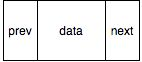
\includegraphics{DLNode.jpeg}
	\caption{Representation of node}
\end{figure}
\paragraph{Implementing Node}
To implement node, we will be making a struct to hold data and the links to store next and previous node . In this implementation we are making a node to store integer type data. However, it can be implemented to store any data type or object.
\begin{lstlisting}
struct Node
{
	int data;
	Node* next;
	Node* prev;
	Node()
	{
		next = NULL;
		prev = NULL;
	}
};
\end{lstlisting}
\paragraph{Initializing the Double linked list}
As a Double linked consists of many nodes, we should have many nodes inside our DLList class, but we will have only two nodes, "head" and "tail", which will act as reference nodes and allows us to iterate through all the nodes in the DLList. Moreover, we will include an integer "length" to keep track of the size of the list.
\begin{lstlisting}
class DLList
{
	private:
		int length;
		Node* head;
		Node* tail;
	public:
		DLList()
		{
			head = NULL;
			tail = NULL:
		}
}
\end{lstlisting}
Our stack now consists of Node pointers which will hold the addresses of the head and the tail. To initialize, both are set to \textbf{NULL}, as the list is empty.
\begin{figure}[H]
	\centering
	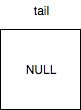
\includegraphics{DLList1.jpeg}
	\caption{DLList head pointer}
\end{figure}
\begin{figure}[H]
	\centering
	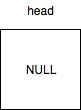
\includegraphics{DLList2.jpeg}
	\caption{DLList tail pointer}
\end{figure}
\paragraph{Implementing Append operation}
Inside the class of DLList, we will declare and define a function "Append(int data)" in public.
\begin{lstlisting}
void Append(int data)
{
	if (length == 0)
	{
		head = tail = new Node();
		head->data = data;
	}
	else
	{
		tail->next = new Node();
		tail->next->prev = tail;
		tail = tail->next;
		tail->data = data;
	}
	length++;
}

\end{lstlisting}
\begin{example}
	Let's visualize an example Append() operation\\
	\begin{lstlisting}
	DLList lst;
	lst.Append(6);
	\end{lstlisting}
	Since the DLList is empty and head is set to NULL. Body of 'if' will be executed.\\
	It first creates a new node and sets head and tail to it.\\
	\begin{figure}[H]
		\centering
		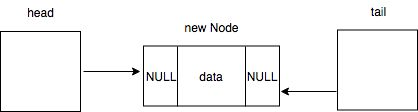
\includegraphics[scale=0.5]{DLList3.jpeg}
		\caption{Creating new node}
	\end{figure}
	~\\
	Then it sets its data to the data passed.
	\begin{figure}[H]
		\centering
		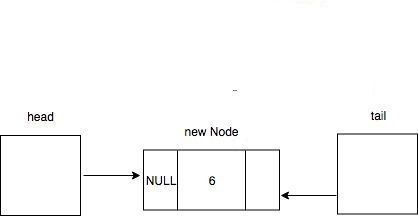
\includegraphics[scale=0.5]{DLList5-set.jpeg}
		\caption{Setting data}
	\end{figure}
\end{example}
Since, length is not '0', Append operation will now execute body of 'else'. Let's see an example
\begin{example}
	\begin{lstlisting}
	lst.append(9);
	\end{lstlisting}
	It will first create a new node and sets tail's next to it.
	\begin{figure}[H]
		\centering
		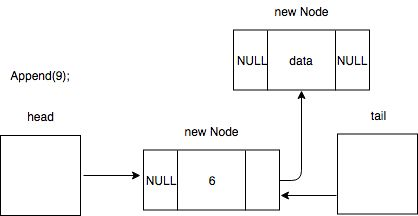
\includegraphics[scale=0.5]{DLList4.jpeg}
		\caption{Creating new node}
	\end{figure} ~\\
	Then it sets the new node's prev to the tail
	\begin{figure}[H]
		\centering
		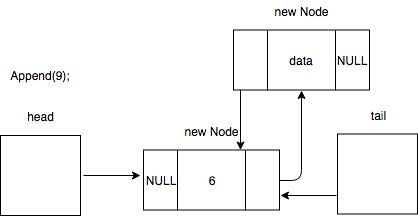
\includegraphics[scale=0.5]{DLList5.jpeg}
		\caption{Setting new node's pointer}
	\end{figure}
	It now updates the tail and sets data.
	\begin{figure}[H]
		\centering
		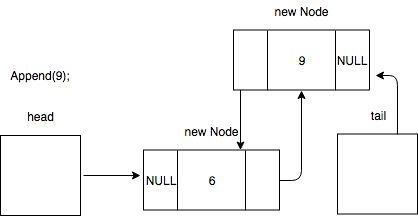
\includegraphics[scale=0.5]{DLList6.jpeg}
		\caption{Updating tail and data}
	\end{figure}
		'9' is added succesfully.
	{\begin{figure}[H]
			\centering
			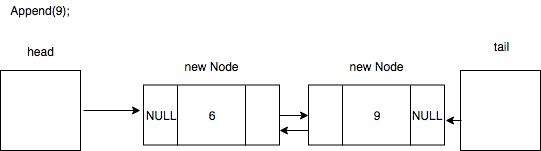
\includegraphics[scale=0.5]{DLList7.jpeg}
			\caption{Succesful Append(9) operation}
	\end{figure}}
\end{example}

\paragraph{Implementing Add operation}
Inside the class of DLList, we will declare and define a function "Append(int data)" in public.
\begin{lstlisting}
void Add(int i, int data)
{
	if(i >= 0 && i <= length)
	{
		if (i == 0)
		{
			if (length == 0)
			{
				head = tail = new Node();
				head->data = data;
			}
			else
			{
				head->prev = new Node;
				head->prev->next = head;
				head = head->prev;
				head->data = data;
			}
			
		}
		else if (i == length)
		{
			tail->next = new Node();
			tail->next->prev = tail;
			tail = tail->next;
			tail->data = data;
		}
		else
		{
			Node* temp;
			if (i <= length/2)
			{
				temp = head;
				for (int j = 0; j < i; j++)
				{
					temp=temp->next;
				}
			}	
			else
			{
				temp = tail;
				for (int j = 0; j < length-i-1; j++)
				{
					temp = temp->prev;
				}
			}
		
			Node* newNode = new Node;
			newNode->data = data;
			newNode->prev = temp->prev;
			newNode->next = temp;
			temp->prev->next = newNode;
			temp->prev = newNode;
			
		}
		length++;
	}
	else
	{
		cout << "Index is out of range" << endl;
	}
}

\end{lstlisting}
\begin{example}
	Let's visualize an example Add() operation\\
	\begin{lstlisting}
	DLList lst;
	lst.Add(0,6);
	\end{lstlisting}
	Since the DLList is empty, Body of 'if (i == 0) and if (length == 0)' will be executed.\\
	It will carry out the same operations carried out in Append function.\\
	It first creates a new node and sets head and tail to it.\\
	\begin{figure}[H]
		\centering
		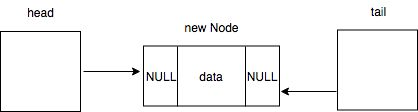
\includegraphics[scale=0.5]{DLList3.jpeg}
		\caption{Creating new node}
	\end{figure}
	~\\
	Then it sets its data to the data passed.
	\begin{figure}[H]
		\centering
		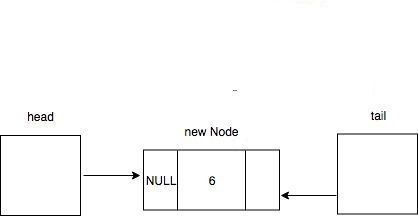
\includegraphics[scale=0.5]{DLList5-set.jpeg}
		\caption{Setting data}
	\end{figure}
\end{example}
If a number is added to the last, it will then also do the same tasks as append.\\

\begin{example}
	\begin{lstlisting}
	lst.Add(1,9);
	\end{lstlisting}
	Now length is not 0 and index is equal to the length.\\
	It will first create a new node and sets tail's next to it.
	\begin{figure}[H]
		\centering
		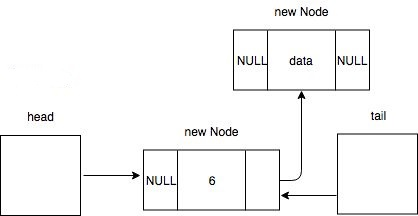
\includegraphics[scale=0.5]{DLList4-add.jpg}
		\caption{Creating new node}
	\end{figure} ~\\
	Then it sets the new node's prev to the tail
	\begin{figure}[H]
		\centering
		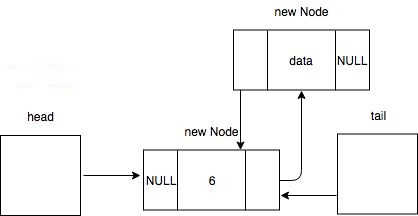
\includegraphics[scale=0.5]{DLList5-add.jpg}
		\caption{Setting new node's pointer}
	\end{figure}
	It now updates the tail and sets data.
	\begin{figure}[H]
		\centering
		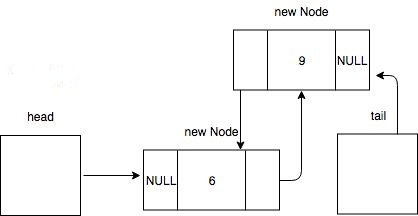
\includegraphics[scale=0.5]{DLList6-add.jpg}
		\caption{Updating tail and data}
	\end{figure}
	'9' is added succesfully.
	{\begin{figure}[H]
			\centering
			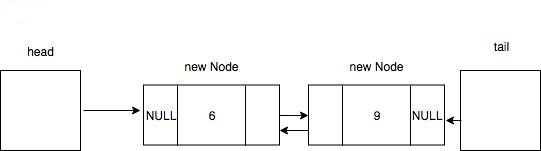
\includegraphics[scale=0.5]{DLList7-add.jpg}
			\caption{Succesful Add(1,9) operation}
	\end{figure}}
\end{example}
\begin{example}
Let's look at an example, when index is neither 0 nor equal to the length.
Let's visualize an example Add() operation\\
\begin{lstlisting}
lst.Add(1,5);
\end{lstlisting}
Since i is less than half of the length, it will iterate from the head.\\
It will first create a temporary pointer and point it to head.
\begin{figure}[H]
	\centering
	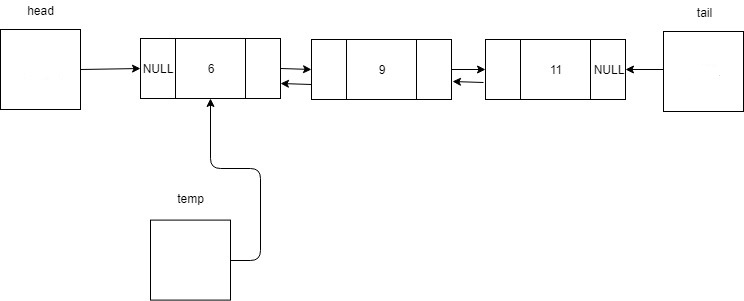
\includegraphics[scale=0.5]{DLAdd1.jpg}
	\caption{Creating a temporary pointer}
\end{figure} ~\\
It will iterate till it reaches the index where a new node is to be added.
\begin{figure}[H]
	\centering
	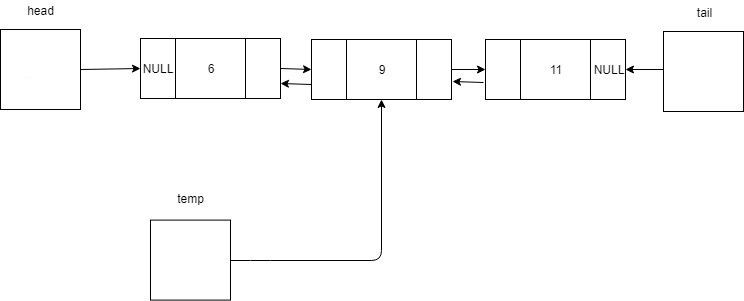
\includegraphics[scale=0.5]{DLAdd2.jpg}
	\caption{Iterating till it reaches the node}
\end{figure}
It will create a new Node.
\begin{figure}[H]
	\centering
	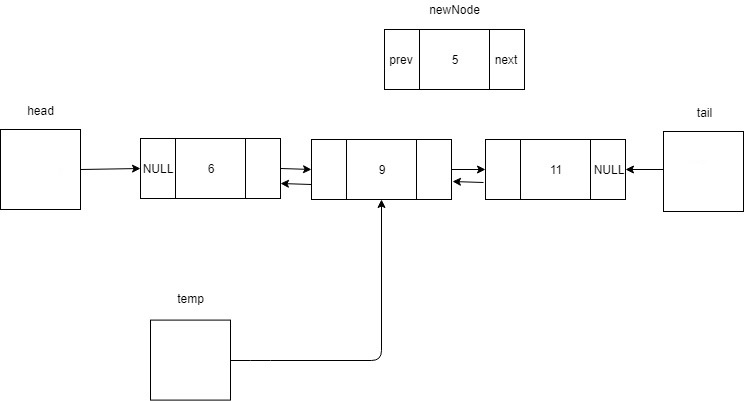
\includegraphics[scale=0.5]{DLAdd3.jpg}
	\caption{Creating new node}
\end{figure}
Points its 'prev' pointer to the temp's 'prev'.
\begin{figure}[H]
	\centering
	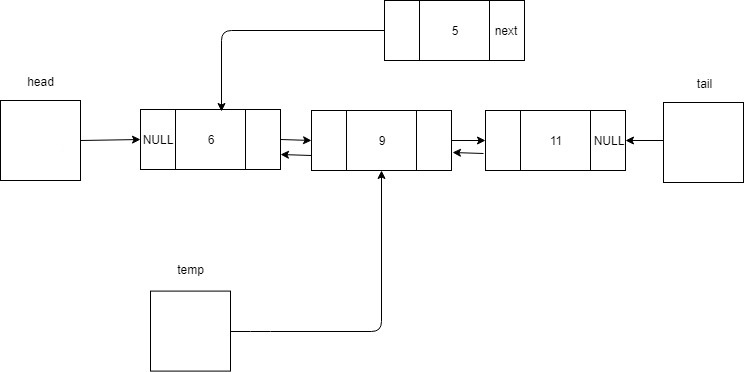
\includegraphics[scale=0.5]{DLAdd4.jpg}
	\caption{Setting node's prev pointer}
\end{figure}~\\
Points its 'next' pointer to temp.
\begin{figure}[H]
	\centering
	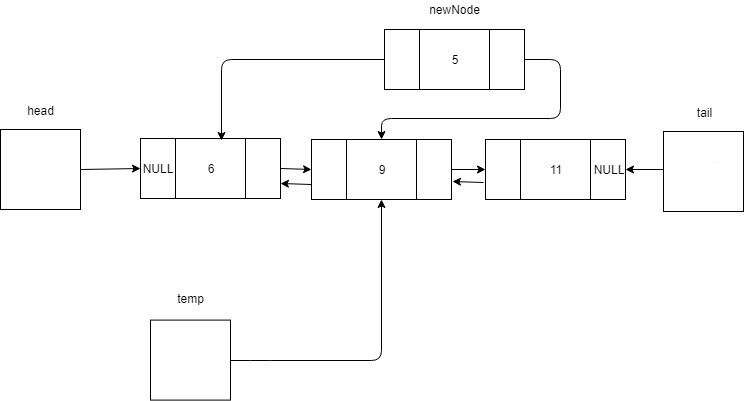
\includegraphics[scale=0.5]{DLAdd5.jpg}
	\caption{Setting node's next pointer}
\end{figure}
Point Node's prev's next pointer to itself.
\begin{figure}[H]
	\centering
	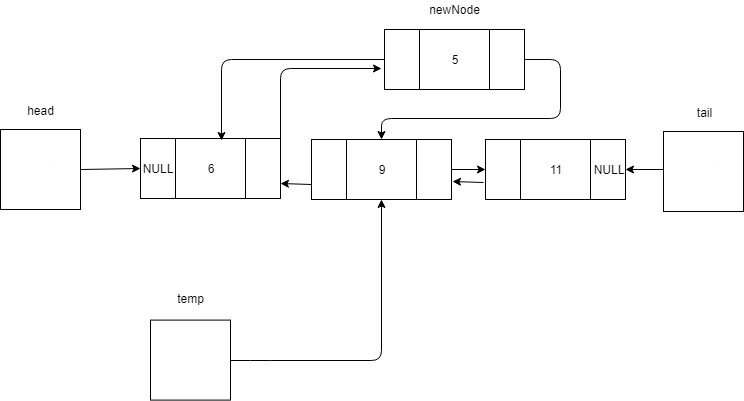
\includegraphics[scale=0.5]{DLAdd5(1).jpg}
	\caption{Setting the previous node's next pointer}
\end{figure}
And finally temp's prev to the new node.
\begin{figure}[H]
	\centering
	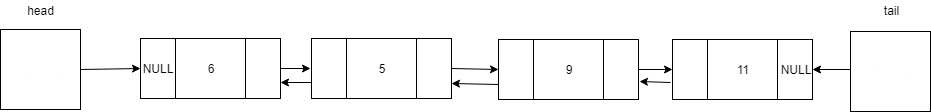
\includegraphics[scale=0.5]{DLAdd6.jpg}
	\caption{Succesful addition}
\end{figure}
\end{example}
\begin{example}
Now, let's see an example where index is greater than the half of the length of the list.\\
\begin{lstlisting}
lst.Add(2,13);
\end{lstlisting}
Since index is greater than the half of the length, it will start iteration from the last.\\
It will first create a temporary pointer and sets it to the tail.
\begin{figure}[H]
	\centering
	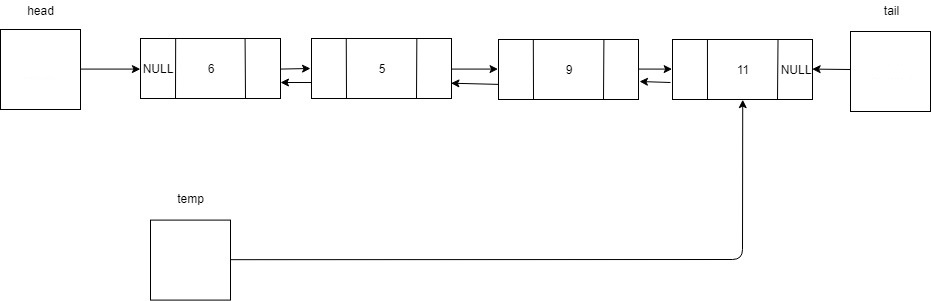
\includegraphics[scale=0.5]{DLAdd7.jpg}
	\caption{Creating a temporary pointer}
\end{figure}
It will iterate till it reaches the index where the new node has to be added
\begin{figure}[H]
	\centering
	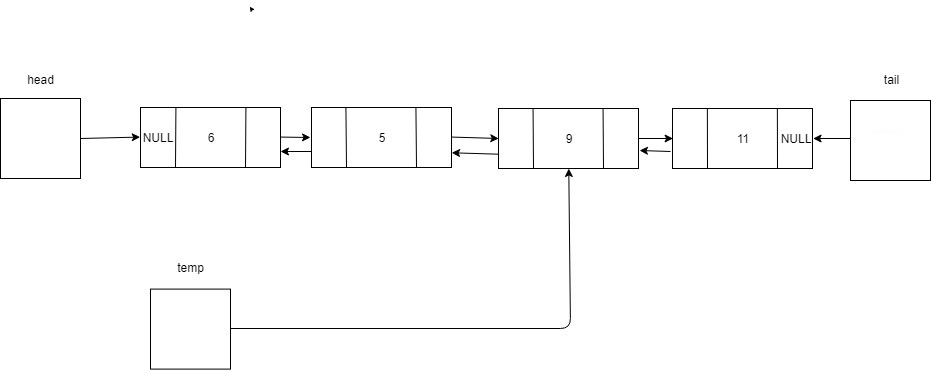
\includegraphics[scale=0.5]{DLAdd8.jpg}
	\caption{Iterated till the index}
\end{figure}
Now it repeats the same process of setting pointers as it did above and adds the new node succesfully.
\begin{figure}[H]
	\centering
	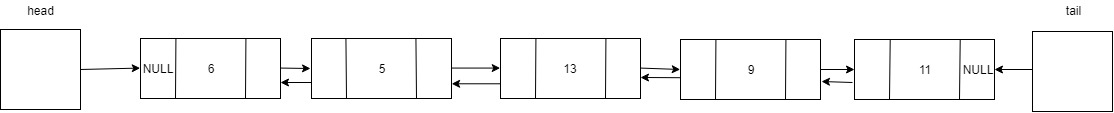
\includegraphics[scale=0.5]{DLAdd10.jpg}
	\caption{Succesful Add(2,13) operation}
\end{figure}
\end{example}
Let's see an example when the length is not '0' and the node is to be added at index '0'.
\begin{example}
	\begin{lstlisting}
	lst.Add(0,4);
	\end{lstlisting}
It will first create a new node and sets the prev's pointer, of the node pointed by head, to it.
\begin{figure}[H]
	\centering
	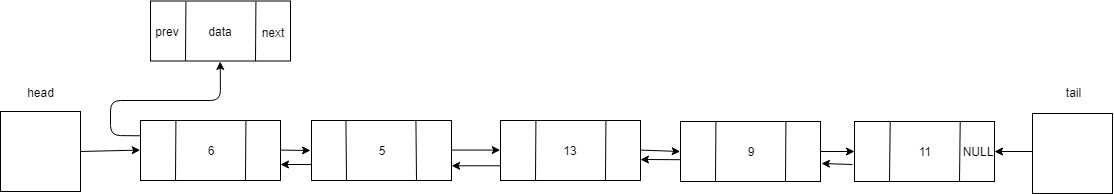
\includegraphics[scale=0.5]{DLAdd11.jpg}
	\caption{Creating new node and setting head's prev}
\end{figure}~\\
Then it sets new node's next to the next of node pointed by head.
\begin{figure}[H]
	\centering
	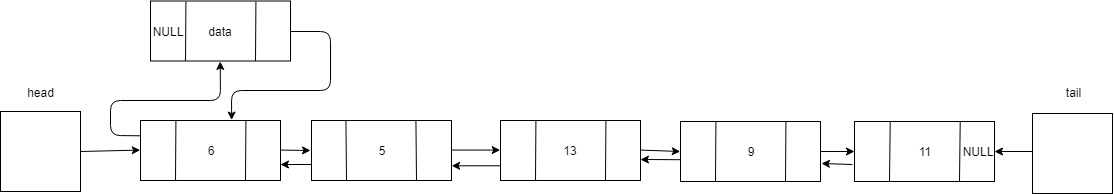
\includegraphics[scale=0.5]{DLAdd12.jpg}
	\caption{Setting node's next pointer}
\end{figure}~\\
Finally, head is set to the new node and the node is added succesfully.
\begin{figure}[H]
	\centering
	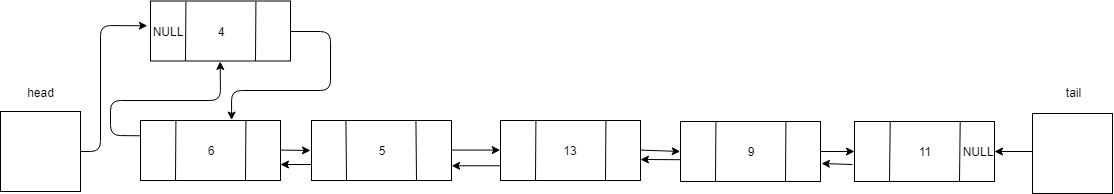
\includegraphics[scale=0.5]{DLAdd13.jpg}
	\caption{Updating head}
\end{figure}
\end{example}
\paragraph{Implementing Show() function}
The Show()  function allows to output all the values in the DLList. \\
Inside the class of DLList, we will declare and define a function "void Show()" in public.
\begin{lstlisting}
void Show()
{
	Node* temp = head;
	while(temp!=NULL)
	{
		std::cout<<temp->data<<std::endl;
		temp = temp->next;
	}
}
\end{lstlisting}
\newpage
Let's visualize an example of Show() operation
\begin{example}
	\begin{lstlisting}
lst.Show();
	\end{lstlisting}~\\
It creates a temp pointer and is pointed to the node pointed by head. It also outputs its value
\begin{figure}[H]
	\centering
	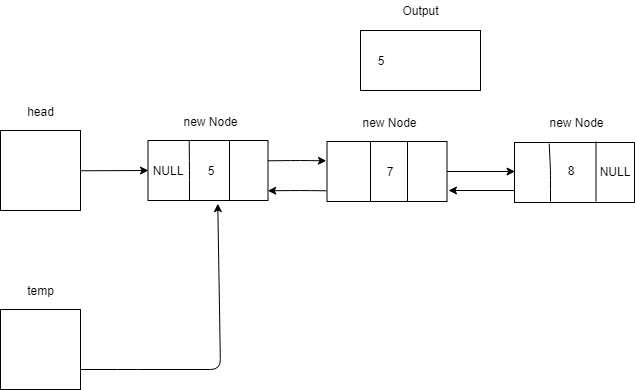
\includegraphics[scale=0.5]{DLShow1.jpg}
	\caption{Creating temp pointer and outputting first value}
\end{figure} ~\\
It updates the temp pointer and moves to the next node. Then it outputs the value of the node pointed by temp.
\begin{figure}[H]
	\centering
	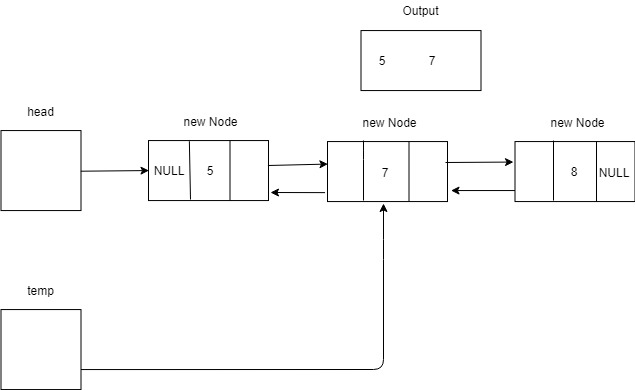
\includegraphics[scale=0.5]{DLShow2.jpg}
	\caption{Outputting second value}
\end{figure}
\newpage
And finally it moves to the last node, outputs its value and since it's next is equal to NULL, the loop is ended.
\begin{figure}[H]
	\centering
	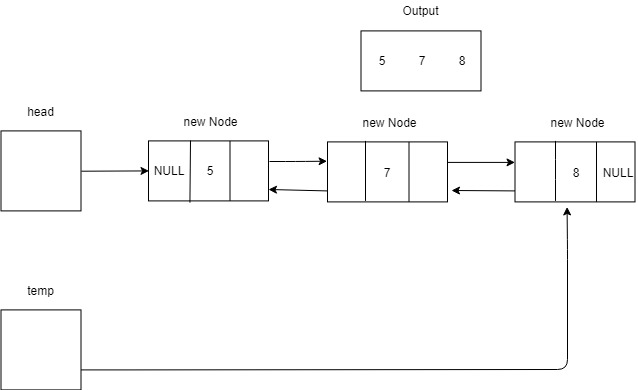
\includegraphics[scale=0.5]{DLShow3.jpg}
	\caption{Outputting third value}
\end{figure} ~\\
\end{example}
\newpage
\section{Problems}\index{Problems}
\begin{problem}
	Implement the Remove(int index) function in your DLList class. The function should remove the element from the given index and returns the removed element. The function should run in O(min(i, n - i)).
	\paragraph{Instructions}
	\begin{itemize}
		\item Think for all special cases such as, removal at zero index and removal at last index.
		\item Update pointers carefully.
		\item Try to take an idea from given Add() function for traversal.
	\end{itemize}
\end{problem}
~\\
\begin{problem}
	Implement the function Reverse() which reverses the list, without making a new list.
	\paragraph{Instructions}
	\begin{itemize}
		\item Traverse through the whole list and update its pointers accordingly
	\end{itemize}
\end{problem}
\newpage
\section{Feedback}\index{Feedback}
\textbf{Please write the things you've learned from this lab and suggestions to make it more better and easy to learn.}
%----------------------------------------------------------------------------------------

\end{document}
